%% IF YOU DON'T HAVE THE MOST RECENT VERSION OF ReVTeX,
%% UNCOMMENT THE APPROPRIATE LINE OF \documentclass
\documentclass[twocolumn,showdate,prd,aps]{revtex4}
%\documentclass[twocolumn,showpacs,amsmath,amssymb,prc,aps]{revtex4-1}
%\documentclass[12pt]{article}
\usepackage{graphicx}
%\usepackage{amssymb}
\usepackage{epstopdf}
%\usepackage{amsthm,  mathrsfs, enumerate, cite}
% \usepackage{amsthm,  mathrsfs, enumerate}
% \usepackage{amsthm,   enumerate}
\usepackage[usenames,dvipsnames]{color}
 
\pdfpagewidth 8.5in
\pdfpageheight 11in 

\topmargin -1cm \textheight 22cm

\setlength\textwidth{6.5in}
\setlength\oddsidemargin{0in}
\setlength\evensidemargin{0in}
\setlength{\parindent}{0.25in}

%\usepackage{amsmath}
%\usepackage{MnSymbol}

%\numberwithin{equation}{section}

\newcommand{\req}[1]{Eq.\,(\ref{#1})}
\newcommand{\reqr}[2]{Eq.\,(\ref{#1}-\ref{#2})}

\begin{document}\hbadness=10000
%%%%%%%%%%%%%%%%%%%%%%%%%%%%%%%%%%
  \hyphenation{strang-en-ess}
%%%%%%%%%%%%%%%%%%%%%%%%%%%%%%%%%%%%%%%%%%%
\title{In the beginning: How matter formed}
\author{Johann Rafelski}
\affiliation{% 
Department of Physics, University of Arizona,
 Tucson, AZ 85721, U.S.A.}
\date{Tucson, September 17, 2013}

\begin{abstract}
How did matter form in the Universe, what is the origin of inertial mass of matter, why are quarks not free,  why is there only matter around us, no antimatter? These are just a few questions that the relativistic heavy ion program at CERN and in US at BNL laboratory investigated, report Vojtech Petracek from CVUT and Johann Rafelski from Tucson, Arizona. They recount here the origin of their research interests. 
\end{abstract}
\vspace{0.8cm}
 
\maketitle

%%%%%%%%%%%%%%%%%%%%%%%%%%%%
For the first 30 $\mu$sec after the Big Bang the early Universe  was a hot soup that contained  the elementary primordial building blocks and in particular the light  quarks now hidden in protons and neutrons, and beyond this electrons, neutrinos,  and even strange quarks we come back to discuss below. Gluons which are akin to photons in that they provide the interaction between color charged quarks were very abundant as well. This primordial phase lasted as long as the temperature of the Universe was more than 100,000 times that expected to prevail in the center of the Sun. 


This view of the early Universe emerged a bit more than 30 years ago. Before, quarks which have been around for a few years were not entering in that discussion in full. However, situation changed when the heavy-ion experimental physics program was developed at CERN in early 1980's.  One of us (JR) was involved in this actively and recollects how this program was justified: as an  opportunity to recreate the primordial form of matter otherwise found only in the early Universe. We argued that in a violent collision of heaviest nuclei an ambient temperature of about  $T\simeq 150$\,MeV$\approx 1.7\, 10^{12}$\,K is reached, the usual matter dissolves into the primordial quark-gluon plasma. The modeled temperature of center of the sun is $1.57 \, 10^{7}$\,K.

Following almost thirty years of difficult and  dedicated relativistic heavy ion experiments at CERN and  in USA at BNL (Brookhaven National Laboratory, Long Island) and,  equally important of parallel theoretical work, interpreting  and guiding these experiments, and providing numerical simulations. One of the authors (VP) leads a CVUT research group working at CERN   within the ALICE collaboration, one of the major LHC experiment. The other among the authors (JR) has been associated with CERN for the past 36 years, and works to interpret the experimental results data from his home base in Tucson, USA.  We interact at CERN, at conferences, prepare joint reports and  publications. The outcome of this research is conviction we share with many others that  the present day knowledge excludes all other options, the results of our work convincingly proves that the Universe before matter was formed was filled with   quark-gluon plasma. In making this discovery we gain many other interesting insights. 

To explain how it is possible that primordial matter has different constituents as compared to matter today we need to make a brief excursion into a better understanding what empty space is exactly. Is the vacuum really empty?  Though devoid of matter, vacuum hosts a new phenomenon made possible by quantum physics, complex quantum fluctuations. This quantum structure of the empty space surrounding us is the cause why  quarks cannot appear as free particles, they are contained inside bubbles we call nucleons. When we compress and heat many quark bubbles, at a temperature high enough   the quantum structure   dissolves allowing quarks to escape  forming  the primordial quark-gluon plasma. 

The theoretical and experimental insight that nucleons are bubbles of quarks confined by the structure of the vacuum to a very small nucleon size volume alters our understanding about the origin of inertial mass of matter. To begin, recall that in the wake of the last year's discovery of the Higgs-(like)particle at CERN, it has become common knowledge that this final building block of   the standard model of particle physics gives to all elementary particles their mass. This said, the mass of matter is not due to the Higgs effect. The quarks from which protons and neutrons are made have a mass more than 100 times smaller than these nucleons. 

The dominant matter mass-giving mechanism  is  popularly called quark confinement. Light quarks are compressed by the quantum vacuum structure into a small space domain  a hundred times smaller than their natural `size'. That costs a lot of energy which is  the nucleon mass. The remaining few percent of mass are than due to the fact that quarks also have inertial mass provided by the Higgs mechanism. Quantitatively, nucleons which  provide practically all the mass of matter derive about 95\%  and in some interpretations up to 99\% of their mass from the interaction of quarks with the confining vacuum.

%%%%%%%%%%%%%%%%%%%%%%%%%%%%%%%%%%%%%%%%
\begin{figure}[!tbh]
\centerline{\includegraphics[width=8cm]{JRMICROBANG2.ps}}
\caption{ %\small
Visualization  of a micro-bang fireball formed in collision of two Lorentz contracted lead nuclei.  The quark-gluon plasma explodes and breaks up into thousands of particles shown as arrows. Also shown  are the physical properties that differ between big-bang and micro-bang: the  
typical lifespan $\tau$\,, which differs by 18 orders of magnitude, and matter antimatter asymmetry which differs by about 6 orders of magnitude.\label{BangComp} 
}
%\vspace*{.6cm}
\end{figure}
%%%%%%%%%%%%%%%%%%%%%%%%%%%%%%%%%%%%%%%%%
 
The conditions in the early universe and those created in relativistic collisions of heavy atomic nuclei differ somewhat: whereas the primordial quark-gluon plasma survived for about 30 $\mu$sec  in the big-bang, the comparable extreme conditions  we create in laboratory in ultra-relativistic nuclear collisions are  expected to prevail for an extremely short blink in time, those of us who are used to count zeros will enjoy the number,  $10^{-22}$\,s. The lifespan in laboratory is limited due to the relativistic explosive disintegration of an extremely hot dense matter drop we created, a relativistic `fireball'. For this reason it is necessary to identify a probe of this deconfined matter that can function within such a short observation time. 

Seeking a diagnostic tool that wins over the short lifespan our research is focused on the understanding of strangeness, the physics of the strange quark. When many years ago in late '50s  some odd experimental results were noted, the new feature  earned that name, which today denotes the  heavier quark.  The great theoretical insight achieved early in the development of the CERN experimental research program was that even in the short time we have,  strangeness will be cooked to a large abundance, one speaks of strangeness thermal equilibrium abundance in quark-gluon plasma. This new feature is the key allowing us to seek, find, observe, evaluate the quark-gluon plasma properties on the time scale that is so immensely short. 

It is at this point important to mention that while for simplicity so far we spoke of only quarks in quark-gluon plasma, there is nearly equal and very high anti-quark, the mirror-quark abundance present. Just like protons are made of three quarks, antiprotons are made of three antiquarks. The hot quark-gluon plasma drop is full of both, quarks and antiquarks.  The total number of quarks and antiquarks is in LHC experiments at CERN a thousand times or even more abundant than the net number of quarks less antiquarks.  Quark-gluon plasma created in laboratory is a phase of matter where matter and antimatter are nearly equally abundant and this symmetry is a million times better in the quark-gluon plasma present in the early Universe. Note, if you ever dreamed to travel to the stars using antimatter propulsion, you will need to find or produce antimatter. An anitmatter factory   will for sure exploit formation of quark-gluon plasma.

This works as follows: the tiny quark-gluon drop, a hot fireball full of this primordial matter, expands and  explodes, it produces many particles we are accustomed to, in a process called `hadronization': the word hadron derived from Greek:  
%ἁδρός, 
hadr\'os, meaning thick, heavy and strong refers to  all strongly interacting particles and antiparticles. As energy contained in the quark-gluon plasma is used up to create matter and antimatter particles  particles, the high abundance of strange quark pairs present in the plasma is preserved and as outcome we observe not only antimatter but also exotic forms  containing strange particles. With time strangeness also decays as it is heavier than the usual quarks and antiquarks. The intermediate presence of strange hadrons  offers us the opportunity to demonstrate that the primordial form of matter was indeed produced, to measure its properties, and to evaluate the time line  of the process. 

%%%%%%%%%%%%%%%%%%%%%%%%%%%%%%%%%%%%%%%%%%%%%%%%%%%
\begin{figure}[tb]
\centerline{\includegraphics[width=8cm]{JRSTRANGEPROD2.ps}}
\caption{ %\small
Schematic representation of strangeness production inside quark-gluon bubble and ensuing hadronization all quarks and antiquarks by recombination into hadrons, showing the exotic $\Xi^0\!(ssu)$  and $\Omega(\bar s\bar s \bar s)$ production as examples. 
\label{hadronize}}
\end{figure}
%%%%%%%%%%%%%%%%%%%%%%%%%%%%%%%%%%%%%%%%%%%%%%%%%%%

One of interesting questions that reverberates in the research program is if the transformation of quark-gluon plasma into normal `hadronic' matter is a phase transition, akin to situation seen in superconductivity, the hot phase is quark conductive, the cold phase is a quark insulator. The drastic change in the local mobility of quarks supports the notion of a phase transition but detailed numerical model computations have in past years changed sides a few times on this issue and now they indicate that there is just a smooth rapid phase transformation, there is no discontinuity in the physical process. This result if past history is a guide could still change. 

One can wonder if it really matters that  we understand such technical detail about the early Universe. And yes, in science such details matter. The Universe has today an unusual asymmetry, all matter around us is matter - no we did not misspeak, what we say is that we do not see antimatter. The question how this is possible excites many discussions. The point to know in our context is that when quark-gluon plasma hadronizes in the early universe, the abundance of matter and antimatter is almost identical. The asymmetry around us is generated by a tiny asymmetry differentiating the number of quarks and antiquarks, at the level of  one in a billion. Moreover, this asymmetry can hide in strangeness which is also at first very abundant in the Universe. Thus one cannot escape the question, do we see matter around us because antimatter is afar and away, separated off in the process of  early universe hadronization, with strangeness helping to separate the two forms of matter? 

While such an idea may sound tentative to some,  it is important to keep in mind that the physics potential exists and has not been yet explored experimentally or theoretically. Other approaches to generate a matter-antimatter asymmetry that   were proposed and modeled are all not fully satisfactory, indeed one could simply say, nothing has so far worked convincingly. The matter asymmetry is an enigmatic riddle of cosmology, of particle physics, and as we now argue, could be part of the physics of quark-gluon plasma and its hadronization transformation into matter. 

So let us conclude by saying  that what we learn about quark-gluon plasma and its hadronization in the laboratory experiment clarifies how matter emerges and particles evolve in the big-bang. We learn to understand how a nearly matter-antimatter symmetric universe is created, from which the present day Universe emerges: In three seconds  all locally available antimatter  annihilates on matter leaving a tiny excess.   While working on this process in laboratory experiments we study the  new physics paradigm, the change in transport properties of the structured quantum vacuum, which depending on temperature allows quarks to move freely in the Universe. In the process we learn about origin of inertial mass which is not what one could think. And as an aside we create know-how how to build an antimatter factory just in case someone wants one -- it does not work the way Dan Brown described it at all in ``Angles and Demons''. But  scientific detail aside, it was fun noting that CERN has also been turned into a movie factory.  Our hands are quite full. 




\end{document}
%%%%%%%%%%%%%%%%%%%%%%%%%%%%
%%%%%%%%%%%%%%%%%%%%%%%%%%%%
%%%%%%%%%%%%%%%%%%%%%%%%%%%%
%%%%%%%%%%%%%%%%%%%%%%%%%%%%






















































